\documentclass[11pt,a4paper]{report}
\usepackage[utf8x]{inputenc}
\usepackage[french]{babel}
\usepackage{ucs}
\usepackage{amsmath}
\usepackage{amsfonts}
\usepackage{amssymb}
\usepackage{graphicx}
\usepackage{geometry}
\usepackage{float}
\usepackage{color}
\usepackage{pdfpages}
\usepackage{listings}

\usepackage[pdftex,
            pagebackref=true,
            colorlinks=true,
            linkcolor=blue,
            unicode
           ]{hyperref}

\title{Apprentissage symbolique avec des r\'eseaux de neurones.}
\author{Corentin Lothod\'e, Pierre Parent, Duy Anh Trinh}

\begin{document}

\maketitle

\tableofcontents

\chapter{Analyse des besoins}
	\section{Objectifs fonctionnels du programme}

	\subsection{Reconnaissance de caractères}

Le but de projet est de réaliser un programme capable de reconnaitre des
caractères en utilisant un réseau de neurones. Nous tenterons de reconnaitre les
caractères 'a' et 'b'. Cela dit le programme sera général et permettra
d'apprendre à distinguer deux caractères quels qu'ils soient.

Les images seront binaires : elles ne contiennent que deux couleurs: noir et blanc. Cela dit il faut remarquer que l'on ne perd pas en généralité en ne choisissant que des images binaires, en effet un filtre bien sélectionn\'e permettrait de se ramener à une image binaire à partir de n'importe quelle image couleur. L’échantillon d'image sera tiré de plusieurs polices de caractère existantes ainsi que de numérisations de nos écritures à la mains sur les quelles il sera réaliser un filtre afin de se ramener à une image binaire. Le filtre pourra être réalisé très facilement via le logiciel
Gimp.

Les images \`a tester auront pour format 30x30 pixels, mais encore une fois nous ne perdons pas en généralité puisqu'un redimensionnement d'image permettra de convertir n'importe quelle image en se format. Un des premier travail de ce projet sera de réfléchir puis de fixer la façon dont les données de l'image seront communiquées à la couche d'entrée des neurones. En effet on peut envisager plusieurs situation : mettre en entrée les pixels de l'image tels quels ou bien réaliser des prétraitement sur l'image, et donner en enter des données déjà traités.

\begin{center}
	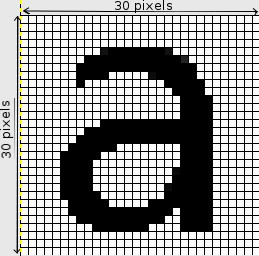
\includegraphics[width=0.66\linewidth]{img/char.png}
\end{center}

La reconnaissance de formes et l'apprentissage dans le domaine de la vision est une application classique des réseaux de neurones, nous pouvons donc espérer réussir à faire marcher , en pratique cette reconnaissance de caractère. De plus nous somme sur de pouvoir trouver de la documentation et de l'aide sur internet puisque ce sujet est assez classique.

	\subsection{Interface du logiciel}

L'interface homme machine du logiciel attendu sera minimaliste et en ligne de
commande. Le logiciel aura deux commandes principales :

\begin{itemize}
	\item \textbf{Lancer la phase d'aprentissage:}	\newline 
%		\textit{neurones -l dossierCarcteres1 dossierCarcteres2[-o neuronesFile]}\newline
		Cette fonctionnalit\'e permettra de r\'ealiser la phase d’apprentissage afin de distinguer les caract\`eres se trouvant sur les images situ\'ees dans un dossier \textit{dossierCaracteres1} de celles situ\'ees dans le dossier \textit{dossierCaracteres2}. Le r\'eseaux de neurones obtenu sera alors stock\'e dans un fichier pour permettre sa r\'eutilisation.
	\item \textbf{Demander une reconnaissance de caract\`ere:} \newline
%		\textit{neurones neuroneFile Limage.bmp}\newline
		L'utilisateur pourra fournir au programme une image. Le programme affichera alors si l'image correspond à un caract\`ere de type 1 ou 2 selon l'apprentissage pr\'ec\'edent.
\end{itemize}
	\section{Description des tests}
	\subsection{Op\'erations de contr\^ole qualit\'e}

Les contr\^oles qualit\'es seront r\'ealis\'es par l'\'equipe de d\'eveloppement (avec les tests unitaires et d'assemblage des diff\'erentes parties du logiciel), puis en r\'ealisant un test global sur l'utilisation du logiciel (tests des diff\'erentes fonctionnalit\'es exig\'ees).

	\subsection{Cycle de vie du projet}
%Chaque attente du client peut être satisfaite ind\'ependamment des autres. 

L'utilisation d'un cycle de vie permettant de d\'evelopper chacun des modules s\'epar\'ement est donc appropri\'ee. Le cycle de vie choise est donc un cycle en V.

\begin{figure}[H]
	\centering
	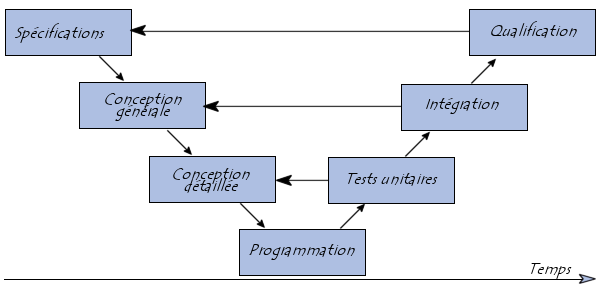
\includegraphics[width=0.66\linewidth]{img/cdv.png} 
\end{figure}

\begin{itemize}
	\item \textit{Sp\'ecifications} : \'etude de l'apprentissage symbolique, son utilisation dans la diff\'erenciation des lettres. 
	\item \textit{Conception g\'en\'erale} : \'etude d\'etaill\'e du programme \`a r\'ealiser, pr\'eparation des tests syst\`emes, des tests d'int\'egration de mise \`a jour des documents \'etablis dans l'\'etape pr\'ec\'edente.
	\item \textit{Conception d\'etaill\'e} : formation de l'architecture interne du programme, d\'efinition des composants, pr\'eparation des tests d'int\'egration et des tests unitaires, mise \`a jour des documents \'etablis dans l'\'etape pr\'ec\'edente.
	\item \textit{Programmation} : codage, documentation des composants.
	\item \textit{Tests:} R\'ealisation des tests, correction du  code si besoin.
	\item \textit{Int\'egration} : l'objectif est de d'assurer la bonne "communication" des diff\'erents modules du programme. Elle fait l'objet de tests d'int\'egration consign\'es dans un document.
	\item \textit{Qualification} : v\'erification de la conformit\'e du logiciel aux sp\'ecifications initiales.
\end{itemize}

\subsection{Gestion de la configuration}
La configuration du programme est compos\'ee des \'el\'ements suivants: le code source ex\'ecutable, les outils de d\'eveloppment, les tests utilis\'es, les documents et les donn\'ees.

Outils de travail collaboratif:
\begin{itemize}
	\item \textbf{SVN}: permet de partager le code source d'un logiciel, de disposer d'un historique de toutes les modifications, et d'int\'egrer facilement les modifications de fichier d'un d\'eveloppeur avant de les mettre \`a disposition des autres utilisateurs.
	\item \textbf{Doxygen}: permet de cr\'eer de la documentation \`a partir
du code source du programme. Pour cela, il tient compte de la grammaire du
langage dans lequel est \'ecrit le code source (ici, C++) ainsi que des
commentaires s'ils sont \'ecrits dans un format particulier.
	\item \textbf{Environnement technique}: le d\'eveloppement sera effectu\'e sous l'environnement GNU/Linux (Ubuntu).
\end{itemize}

\subsection{Gestion des modifications}
Les modifications peuvent avoir deux origines:
\begin{itemize}
	\item d\'etection d'une anomalie: il faut en trouver la source puis la corriger dans le plus bref d\'elai,
	\item demande d'\'evolution: il faut dans un premier temps r\'ealiser un \'etude de faisabilit\'e, pour ensuite modifier le programme en cons\'equence si cela s'av\`ere r\'ealisable dans les d\'elais impartis.
\end{itemize}

	\section{Pr\'esentation des r\'eseaux de neurones artificiels}

	\subsection{Origine}

Ce sont les neurologues Warren McCulloch et Walter Pitts qui les premiers publi\`erent des travaux sur les r\'eseaux de neurones \`a la fin des ann\'ees 1950. Un mod\`ele simplifi\'e est alors introduit, avec la notion de neurone formel. Le neurone somme ses entr\'ees (avec des coefficients synaptiques) et r\'epond si la somme r\'esultante est sup\'erieur \`a un seuil. Ces r\'eseaux de neurones peuvent th\'eoriquement r\'ealiser des fonctions logiques, arithm\'etiques et symboliques complexes. N\'eanmoins, ces travaux ne pr\'ecisent pas comment faire \'evoluer ces coefficients.

C'est le physiologiste Donal Hebb qui donna un d\'ebut de r\'eponse concernant la modification des coefficients synaptiques. Hebb d\'ecrit en 1949 une r\`egle simple qui permet de modifier la valeur des coefficents synaptiques en fonction de l'activit\'e des unit\'es qu'ils relient.

En 1957, Franck Rosenblatt d\'ecrit le mod\`ele du perceptron. C'est le premier syst\`eme artificiel capable d'apprendre par exp\'erience, m\^eme si des erreurs sont commises. En 1969, Marvin Lee Minsky et Seymour Papert publi\`erent un ouvrage montrant l'impossibilit\'e de traiter des probl\`emes non lin\'eaires avec de tels r\'eseaux. L'industrie s'en d\'etourna et la recherche perdit une grande partie de ses financements.

En 1986, c'est le mod\`ele du Perceptron Multi-Couche, propos\'e par Werbos, Rumerhart et Yann le Cun ind\'ependamment. Ces syst\`emes reposent sur la r\'etropropagation de l'erreur. Ils permettent de traiter avec succ\`es des ph\'enom\`enes non-lin\'eaires.

	\subsection{Utilit\'e}

Les domaines d'applications sont notamment :
\begin{itemize}
	\item classification d'esp\`eces animales par analyse ADN,
	\item reconnaissance de motif (notamment de caract\`eres : OCR),
	\item approximation d'une fonction inconnue, mod\'elisation acc\'el\'er\'ee d'une fonction connue,
	\item estimation boursi\`ere,
	\item m\'et\'eorologie.
\end{itemize}

	\subsection{Principe de fonctionnement}

		\subsubsection{Structure du r\'eseau}

Un r\'eseau de neurone est compos\'e d'une succession de couches dont chacune prend ses entr\'ees sur les sorties de la couche pr\'ec\'edente.

\begin{figure}[H]
	\centering
	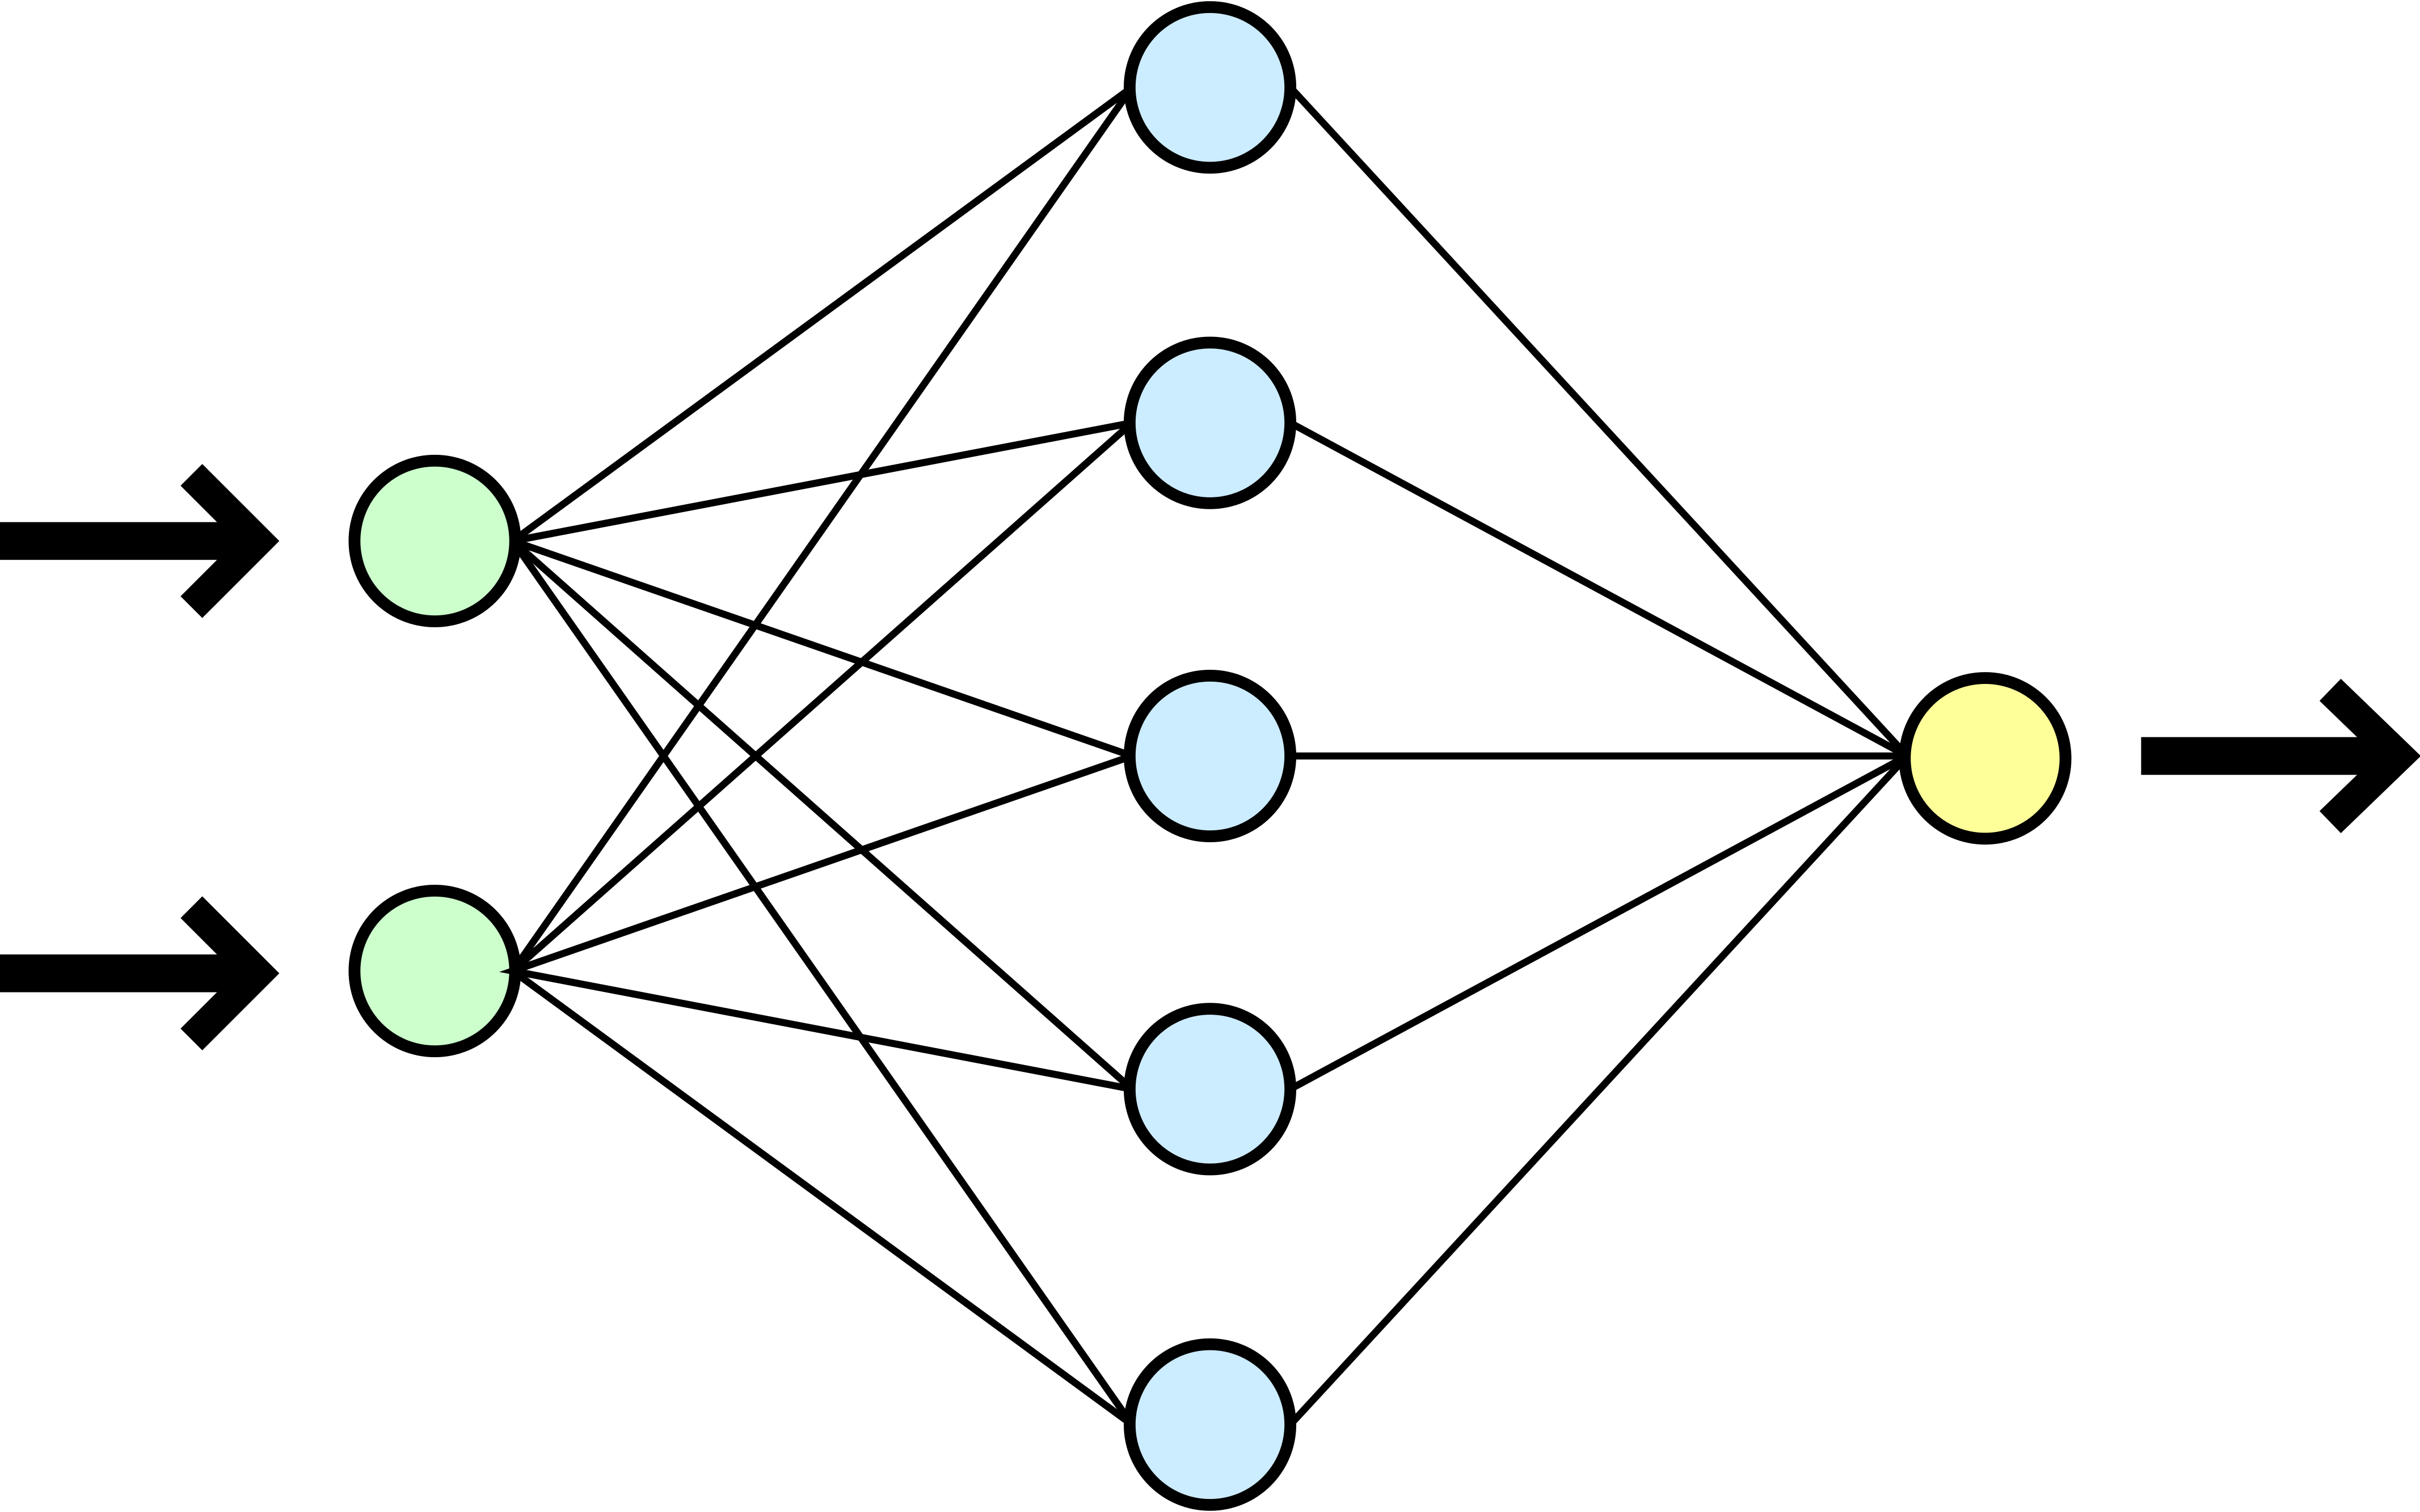
\includegraphics[width=0.66\linewidth]{img/Neural_network.png} 
	\caption{Exemple d'un r\'eseau de neurones avec deux entr\'ees.}
	\label{neurone_ex}
\end{figure}

		\subsubsection{Calcul de la sortie}

\begin{figure}[H]
	\centering
	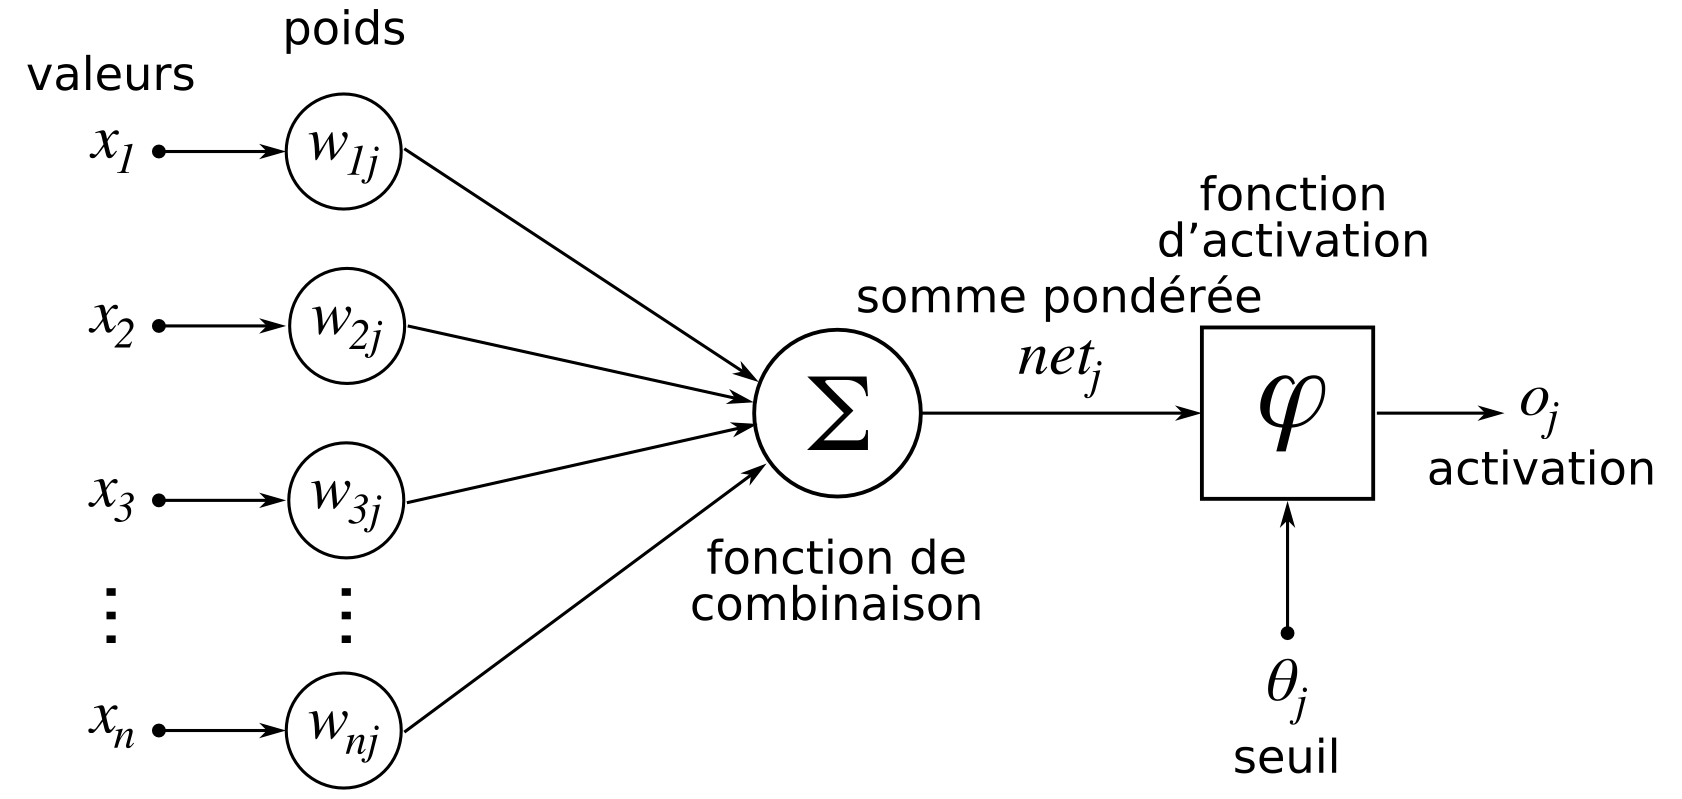
\includegraphics[width=0.66\linewidth]{img/NeuronModel.png} 
	\caption{Fonctionnement sch\'ematique d'un neurone artificiel.}
	\label{neurone_schema}
\end{figure}

Le calcul de la sortie s'effectue selon le sch\'ema explicatif de la figure \ref{neurone_schema}.

		\subsubsection{Fonction de combinaison}

La fonction de combinaison, $\Sigma : \mathbb{R}^n \rightarrow \mathbb{R}$, re\c coit en amont un certain nombre de valeurs via ses connexions synaptiques et retourne un scalaire suivant deux principaux paradigmes :
\begin{itemize}
	\item une combinaison lin\'eaire des entr\'ees (r\'eseaux de type Multi-Layer Perceptron) : $\Sigma(x) = (x,w)$,
	\item la distance entre les entr\'ees (r\'eseaux de type Radial Basis Function).
\end{itemize}

		\subsubsection{Fonction d'activation}

La fonction d'activation sert \`a introduire une non-lin\'earit\'e dans le fonctionnement du reurone. Les fonctions pr\'esentent g\'eneralement trois intervalles :
\begin{itemize}
	\item en dessous du seuil, le neurone est non-actif (sortie \`a $0$ ou $-1$),
	\item aux alentours du seuil, une phase de transition,
	\item au dessus du seuil, le neurone est actif (sortie \`a $1$).
\end{itemize}

Des fonctions classiques de fonctions d'activations sont :
\begin{itemize}
	\item la fonction sigmo\"ide : $f(x)=\frac{1}{1+e^{-\lambda x}}$,
	\item la fonction tangente hyperbolique : $th(x)=\frac{e^x-e^{-x}}{e^x+e^{-x}}$,
	\item la fonction de Heaviside $H(x)=\left\{\begin{matrix} 0 & \mathrm{si} & x < 0 \\ 1 & \mathrm{si} & x \ge 0 \end{matrix}\right.$
\end{itemize}

	\subsection{Apprentissage}

L'apprentissage impliqu\'e dans ces r\'eseaux appartiennent \`a la famille des apprentissages supervis\'es : afin d'amener le r\'eseau \`a avoir le comportement que l'on souhaite, on indique des directions pour am\'eliorer le r\'eseau en donnant des exemples pour lesquels on conna\^it la r\'eponse souhait\'ee.

Un algorithme tr\`es utilis\'e dans ce type d'apprentissages est la r\'etropropagation du gradient (ou encore en anglais backpropagation). Il a pour but de converger de mani\`ere it\'erative vers une configuration optimis\'ee des poids synaptiques.

Soit une entr\'ee $\vec{x}$ et le r\'esultat attendu $\vec{t}$. On propage le signal (gr\^ace \`a la fonction d'activation $g$ et la fonction d'agr\'egation $h$) jusqu'au r\'esultat $\vec{y}$. Pour chaque neurone $i$ dans la couche de sortie, on calcule :
$$e_i^{(s)}=g'(h^{(s)})(t_i-y_i)$$

On propage l'erreur vers l'arri\`ere $e_i^{(n)} \mapsto e_j^{(n-1)}$ gr\^ace \`a la formule suivante :
$$e_j^{(n-1)} = g'^{(n-1)}(h_j^{(n-1)})\sum_i w_{ij}e_i^{(n)}$$

On note :
$$e_j^{(n)} = \sum_i [t_i - y_i] \frac{\partial y_i}{\partial h_j^{(n)}}$$

Enfin, on met \`a jour les poids synaptiques $w_{ij}$ dans toutes les couches :
$$\Delta w_{ij}^{(n)} = \lambda e_i^{(n)}x_j^{(n-1)}$$

o\`u $\lambda$ repr\'esente le taux d'apprentissage (de faible magnitude et inf\'erieur \`a $1$).

\chapter{Sp\'ecifications fonctionnelles}
	\section{Module interface}
Ce module permettra la gestion de l'interface entre l'utilisateur et le programme de reconnaissance de caract\`ere. Il offrira un menu en ligne de commande afin de guider l'utilisateur dans les diff\'erentes possibilit\'es offertes par le logiciel.

Il permettra notamment de :
\begin{itemize}
	\item \textit{voir diagramme de cas d'utilisations}
\end{itemize}

\ \newline Le menu en ligne de commande contiendra 2 choix possibles: Apprentissage et Reconnaissance. Dans chaque choix, on peut trouver encore des options possibles. Par exemple dans l'apprentissage, il y a "Charger Image", "Apprendre" ou "Sauvegarder le r\'ecdseau neurones", et dans Reconnaissance ce sont "Charger Image", "Charger réseau", "Reconnaissance" et finalement "Afficher les r\'esultat". Ce sont tous les fonctions dans les autres modules. 
	\section{Module traitement des entr\'ees}
Ce module aura pour objectif de charger des données à partir d'images au format Bmp, et de mettre en forme ces données afin quelle soient directement traitable par un réseau de neurones. 

	\section{Module r\'eseau de neurones}
Ce module permettra la reconnaissance de caract\`eres gr\^ace \`a un r\'eseau de neurone. Il permettra donc d'effectuer les fonctionnalit\'es de reconnaissance et d'apprentissage. Il permettra l'impl\'ementation de r\'eseaux multicouches, avec diff\'erentes fonctions d'activations.
	\section{Mod\'elisation UML}

	\subsection{Cas d'utilisations}

\begin{figure}[H]
	\centering
	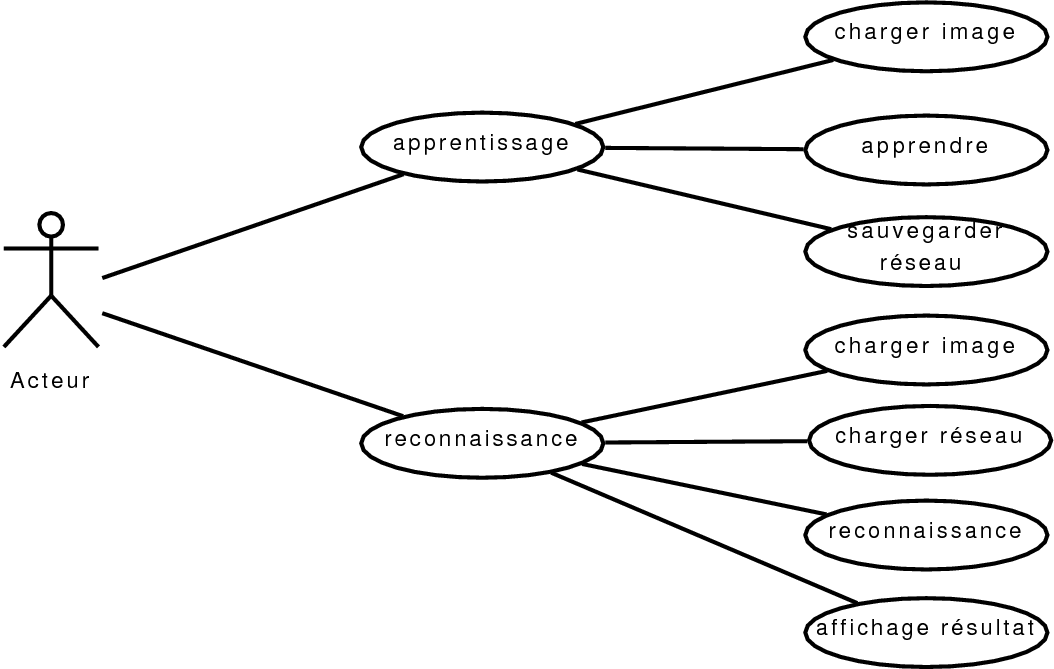
\includegraphics[width=0.8\linewidth]{diag/cas_utilisations.png}
\end{figure}

	\subsection{Modules}

\begin{figure}[H]
	\centering
	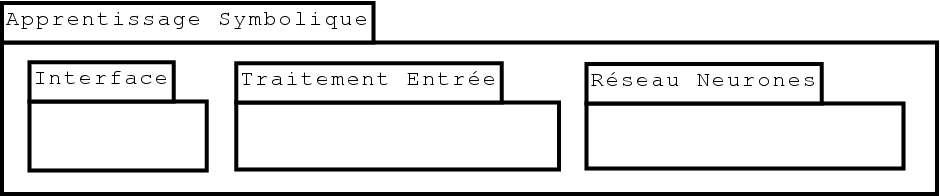
\includegraphics[width=0.8\linewidth]{diag/diag_package.png}
\end{figure}

	\subsubsection{Module Traitement Entr\'ees}

\begin{figure}[H]
	\centering
	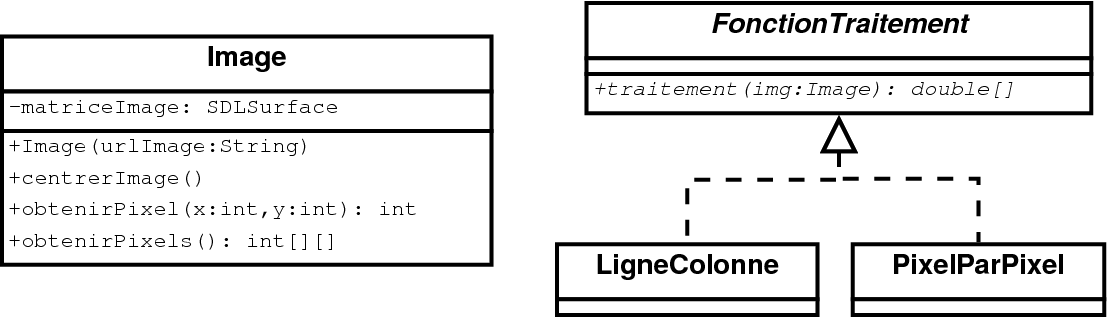
\includegraphics[width=0.7\linewidth]{diag/class_image.png}
\end{figure}

	\subsubsection{Module R\'eseau Neurones}
	
\begin{figure}[H]
	\centering
	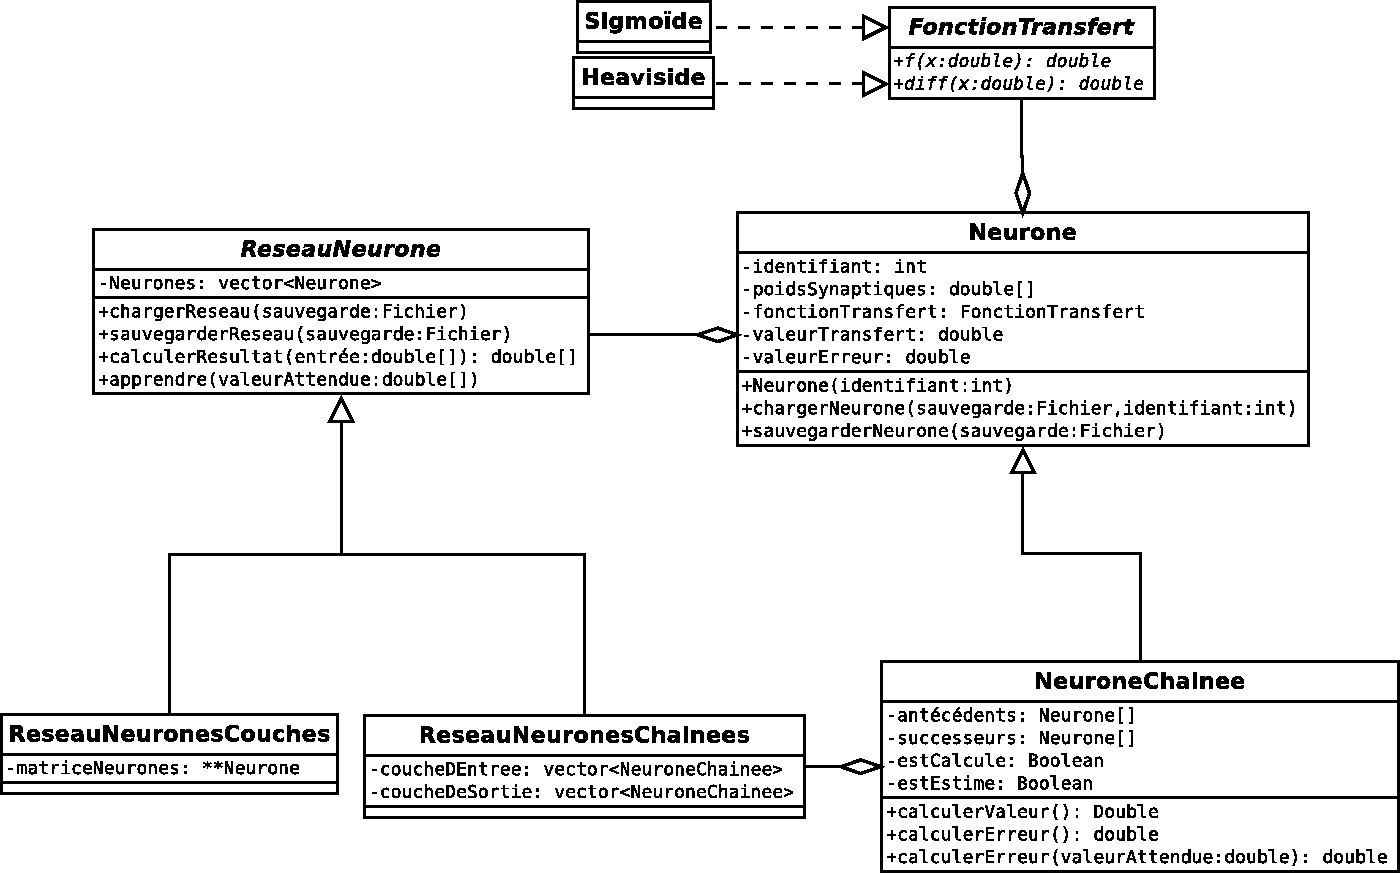
\includegraphics[width=1\linewidth]{diag/class_neurone.png}
\end{figure}

	\subsubsection{Module Interface}
	
\begin{figure}[H]
	\centering
	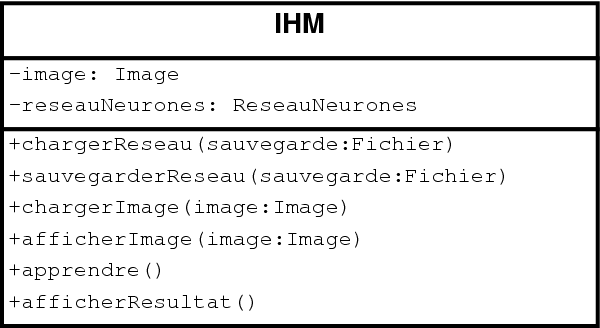
\includegraphics[width=0.4\linewidth]{diag/class_vue.png}
\end{figure}

	\subsection{Diagramme de séquence}

		\subsubsection{Apprentissage}
\begin{figure}[H]                                                                                                    
        \centering                                                                                                   
        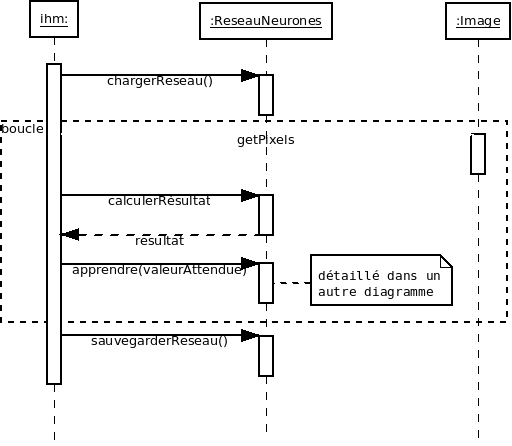
\includegraphics[width=0.6\linewidth]{diag/seq_apprentissage.png}                                                  
\end{figure}

		\subsubsection{Reconnaissance}
\begin{figure}[H]                                                                                                    
        \centering                                                                                                   
        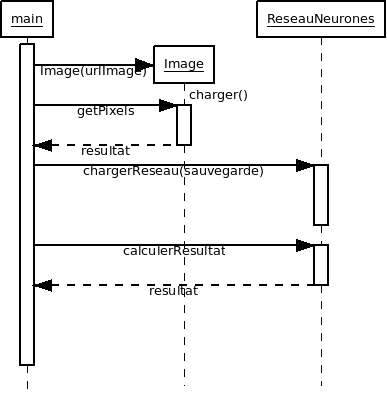
\includegraphics[width=0.6\linewidth]{diag/seq_reconnaissance.png}                                                  
\end{figure}

		\subsubsection{A continuer}
	\section{Préparation des tests d'intégrations}
	
	\subsection{Test de chargement et de traitement de l'image}

Il s'agira de charger une image dont on connait les caract\'eristiques et v\'erifier que l'ensemble des m\'ethodes retournent les bonnes caract\'eristiques. Cela v\'erifie la bonne coordination entre les fonctions qui permettent de charger l'image et celles qui permettent de la traiter, et le bon fonctionnement global du module de gestion des donn\'ees.

	\subsection{Test d'ex\'ecution du r\'eseau de neurones}

On construira un r\'eseau de neurones simple dont on simulera l'ex\'ecution \`a la main et on v\'erifiera alors que l'ex\'ecution en machine via notre programme du r\'eseau de neurone am\`ene au bon r\'esultat. Cela permet de tester la bonne int\'egration des classes neurones, reseaux de neurones, ainsi que la bonne int\'eration entre les différent neurones.

	\subsection{Test de l'apprentissage}

Il va falloir tester si un r\'eseaux de neurones est significativement capable d'apprendre. Pour cela il faudra que l'on ait un jeu de donn\'ee fiable que l'on utilisera pour effectuer une phase d'aprentissage, puis on v\'erifiera que l'apprentissage s'est bien d\'eroul\'e  en utilisant un jeu de donn\'ees test et en v\'erifiant que les r\'esultats donn\'ees par le r\'eseaux de neurones sage sont convainquants. On peut se fixer par exemple l'objectif que 95 \% des instances du jeu de donn\'ees test soient bien class\'ees.

	\subsection{Test de l'interface}

Ce test permmetra de v\'erifier que la navigation dans les menus se fait convenablement et que les bonnes fonctionalit\'es sont appel\'ees lorsque les choix sont valid\'es.

\chapter{Documentation}
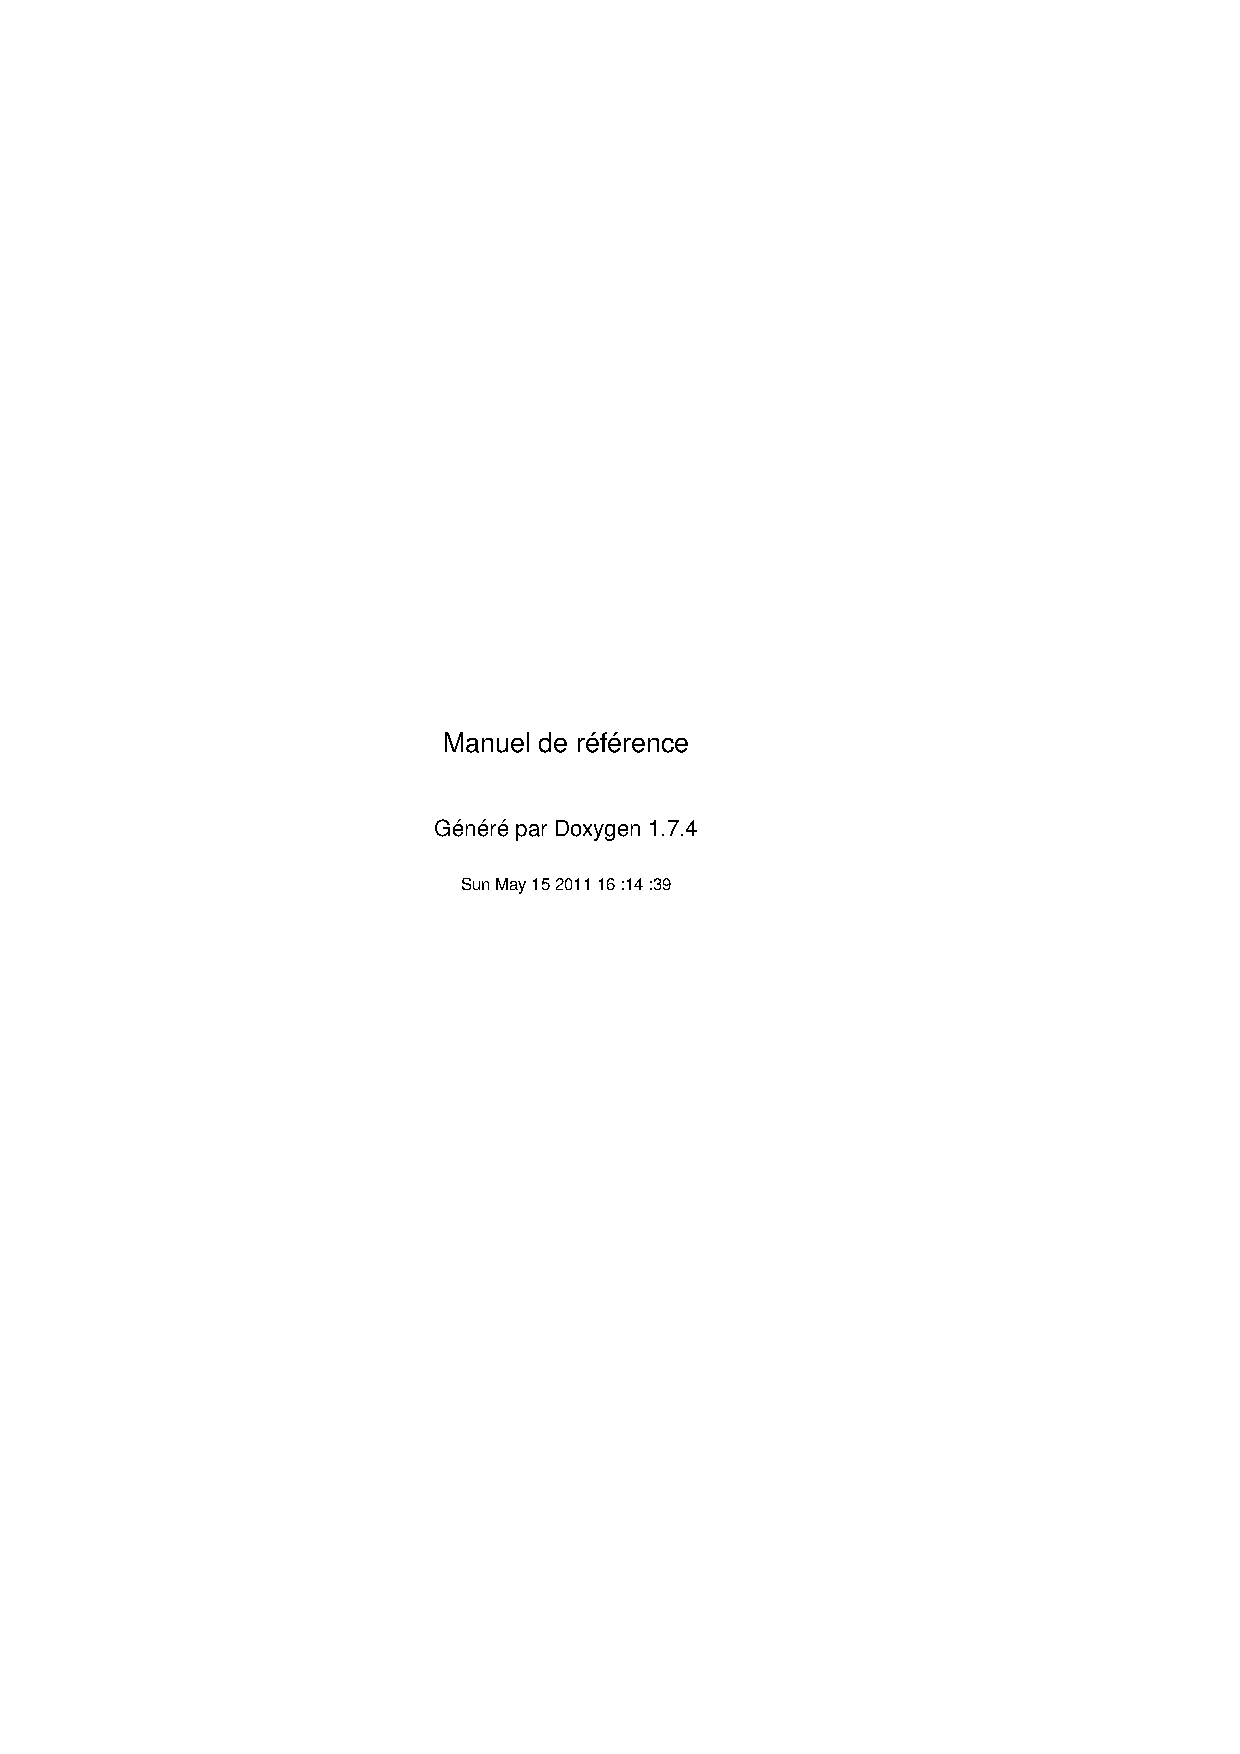
\includepdf[pages = {1-25}]{../doc/latex/refman.pdf}

\chapter{Tests}
	\input{tests.tex}

\chapter{IHM}
	%\documentclass[11pt,a4paper]{report}
%\usepackage[utf8]{inputenc}
%\usepackage{amsmath}
%\usepackage{amsfonts}
%\usepackage{amssymb}
%\usepackage{graphicx}
%\usepackage{geometry}
%\usepackage{float}
%\begin{document}

\section{Le menu principal}
Le menu principal va afficher tout les fonctions principales du programmes. Il s'agit de: \newline

\fbox{
\begin{minipage}{1\textwidth}
Projet C++: Réseaux Neurones \newline

====================== MENU =================== \newline
1. Mode Automatique\newline
2. Apprentissage\newline
3. Reconnaissance\newline
0. Quitter\newline
\end{minipage}}

\section{Mode automatique}
Si le choix est 1, le programme tourne avec es param\`etres par défaut. On a un ensemble d'image a et b qui est donné, et on va tester si on peut les différencier.

\begin{verbatim}
Faire tourner le programme avec les paramètres par défaut()
Apprentissage du jeu d'images A B contenant 30 images
15 premières images attendent A en réponse, les 15 dernières B
Apprentissage
0%
0.833333%
...
98.3333%
99.1667%
---------Echantillon d'apprentissage-----------
A a Image appr 0 :0.992383 Image appr 0 :-0.992422 
A a Image appr 1 :0.992364 Image appr 1 :-0.992361 
...
A a Image appr 22 :0.975503 Image appr 22 :-0.975471 
A a Image appr 23 :0.971372 Image appr 23 :-0.971625 
B b Image appr 24 :-0.989786 Image appr 24 :0.989907 
B b Image appr 25 :-0.980391 Image appr 25 :0.980473 
...
B b Image appr 47 :-0.990786 Image appr 47 :0.990857 
B b Image appr 48 :-0.993504 Image appr 48 :0.993523 
Ouverture du fichier de sauvegarde
Fermeture du fichier de sauvegarde
---------Echantillon de test-----------
B b ok ;) Image test 0 :-0.991597 Image test 0 :0.991683 
A a ok ;) Image test 1 :0.466849 Image test 1 :-0.467163 
A a ok ;) Image test 2 :0.119832 Image test 2 :-0.122299 
B b ok ;) Image test 3 :-0.988773 Image test 3 :0.988838 
A a ok ;) Image test 4 :0.986736 Image test 4 :-0.986759 
A a ok ;) Image test 5 :0.914367 Image test 5 :-0.914328 
A a ok ;) Image test 6 :0.0387813 Image test 6 :-0.0386743 
B b ok ;) Image test 7 :-0.986668 Image test 7 :0.986764 
B b ok ;) Image test 8 :-0.9753 Image test 8 :0.975194 
A a ok ;) Image test 9 :0.793187 Image test 9 :-0.794556 
A a ok ;) Image test 10 :0.791338 Image test 10 :-0.792993 
A a ok ;) Image test 11 :0.972948 Image test 11 :-0.973066 
A a ok ;) Image test 12 :0.992915 Image test 12 :-0.992907 
A a ok ;) Image test 13 :0.930262 Image test 13 :-0.930265 
B b ok ;) Image test 14 :-0.491248 Image test 14 :0.493489 
\end{verbatim}

%\fbox{
%\begin{minipage}{1\textwidth}
%Choix : 1\newline
%=============================================== \newline
%
%faire tourner le programme avec des parametres par défaut() \newline
%Apprentissage du jeu d'images A B contenant 30 images\newline
%15 premiére image attendent A en réponse, les 15 dérniéres B\newline
%Nombre de couches 4\newline
%---------Echantillon d'apprentissage-----------\newline
%A a Image appr 0 :0.992383 Image appr 0 :-0.992422\newline 
%A a Image appr 1 :0.992364 Image appr 1 :-0.992361 \newline
%A a Image appr 2 :0.99349 Image appr 2 :-0.993516 \newline
%A a Image appr 3 :0.992037 Image appr 3 :-0.992066 \newline
%A a Image appr 4 :0.990245 Image appr 4 :-0.990282 \newline
%A a Image appr 5 :0.988849 Image appr 5 :-0.98887 \newline
%A a Image appr 6 :0.98541 Image appr 6 :-0.985357 \newline
%A a Image appr 7 :0.990105 Image appr 7 :-0.990144 \newline
%A a Image appr 8 :0.984867 Image appr 8 :-0.984845 \newline
%A a Image appr 9 :0.98159 Image appr 9 :-0.98165 \newline
%A a Image appr 10 :0.974303 Image appr 10 :-0.974481\newline 
%A a Image appr 11 :0.971432 Image appr 11 :-0.971355\newline 
%A a Image appr 12 :0.976854 Image appr 12 :-0.976665\newline 
%A a Image appr 13 :0.972767 Image appr 13 :-0.972724\newline 
%A a Image appr 14 :0.979867 Image appr 14 :-0.980029\newline 
%A a Image appr 15 :0.97219 Image appr 15 :-0.971962 \newline
%A a Image appr 16 :0.989196 Image appr 16 :-0.989245\newline 
%A a Image appr 17 :0.991669 Image appr 17 :-0.991661\newline 
%A a Image appr 18 :0.982455 Image appr 18 :-0.98239 \newline
%A a Image appr 19 :0.989519 Image appr 19 :-0.98952 \newline
%A a Image appr 20 :0.980113 Image appr 20 :-0.980542\newline 
%A a Image appr 21 :0.992943 Image appr 21 :-0.992982\newline 
%A a Image appr 22 :0.975503 Image appr 22 :-0.975471\newline 
%A a Image appr 23 :0.971372 Image appr 23 :-0.971624\newline 
%B b Image appr 24 :-0.989786 Image appr 24 :0.989907\newline 
%B b Image appr 25 :-0.980391 Image appr 25 :0.980473\newline 
%B b Image appr 26 :-0.979724 Image appr 26 :0.979869\newline 
%B b Image appr 27 :-0.987759 Image appr 27 :0.987935\newline 
%B b Image appr 28 :-0.989009 Image appr 28 :0.989028\newline 
%B b Image appr 29 :-0.991693 Image appr 29 :0.991762\newline 
%B b Image appr 30 :-0.982201 Image appr 30 :0.982077\newline 
%B b Image appr 31 :-0.993486 Image appr 31 :0.993517\newline 
%B b Image appr 32 :-0.990494 Image appr 32 :0.990465\newline 
%B b Image appr 33 :-0.981015 Image appr 33 :0.980937\newline 
%B b Image appr 34 :-0.974582 Image appr 34 :0.974495\newline 
%B b Image appr 35 :-0.983483 Image appr 35 :0.983359\newline 
%B b Image appr 36 :-0.988139 Image appr 36 :0.988225\newline 
%B b Image appr 37 :-0.98496 Image appr 37 :0.985107 \newline
%B b Image appr 38 :-0.975069 Image appr 38 :0.975116\newline 
%B b Image appr 39 :-0.979455 Image appr 39 :0.979357\newline 
%B b Image appr 40 :-0.97496 Image appr 40 :0.975017 \newline
%B b Image appr 41 :-0.975214 Image appr 41 :0.975062\newline 
%B b Image appr 42 :-0.970069 Image appr 42 :0.970275\newline 
%B b Image appr 43 :-0.992843 Image appr 43 :0.992881\newline 
%B b Image appr 44 :-0.985963 Image appr 44 :0.986048\newline 
%B b Image appr 45 :-0.978272 Image appr 45 :0.978077\newline 
%B b Image appr 46 :-0.991868 Image appr 46 :0.991927\newline 
%B b Image appr 47 :-0.990786 Image appr 47 :0.990857\newline 
%B b Image appr 48 :-0.993504 Image appr 48 :0.993523\newline 
%\end{minipage}} \newline

\section{Apprentissage}
%\textbf{Choix 2 : Apprentissage}\newline
Si le choix est 2, le programme utilise le jeu d'apprentissage pour générer un nouveau réseau, et sauvegarde le réseau dans un fichier au choix.

\begin{verbatim}
Apprendre et sauvegarder le réseau
Entrer l'addresse de l'image
img/appr_a1.bmp
Entrer l'addresse souhaitée où l'on sauvegarde le réseau
res/test.txt
Apprentissage
0%
0.833333%
...
98.3333%
99.1667%
Ouverture du fichier de sauvegarde
Fermeture du fichier de sauvegarde
Votre réseau est sauvegardé à l'adresse res/test.txt
\end{verbatim}

%\fbox{
%\begin{minipage}{1\textwidth}
%======================= MENU ===================\newline
%
%1. Mode Automatique\newline
%2. Apprentissage\newline
%3. Reconnaissance\newline
%0. Quitter\newline
% 
%Choix : 2               \newline  
%================================================ \newline
%
%Apprendre et sauvegarder le reseau \newline
%Entrer l'addresse de l'image \newline
%img/appr\_a1.bmp \newline
% Entrer l'addresse souhaite ou on sauvegarde le reseau \newline
%res/test.txt \newline
%Apprentissage\newline
%Ouverture du fichier de sauvegarde  \newline
%Fermeture du fichier de sauvegarde \newline
% Votre reseau est sauvegarde a res/resultat.txt \newline
%\end{minipage}} \newline

\section{Reconnaissance}
Enfin, pour le choix numéro 3, le programme propose de reconnaitre un caractère.
\begin{verbatim}
Reconnaissance
Entrer l'addresse de l'image
img/appr_a1.bmp
Entrer un réseau
res/test.txt
Nombre de couches 4
C'est le caractère numéro :1 (a)
\end{verbatim}

%\fbox{
%\begin{minipage}{1\textwidth}
%======================= MENU ===================\newline
%
%1. Mode Automatique\newline
%2. Apprentissage\newline
%3. Reconnaissance\newline
%0. Quitter\newline
%  
%Choix : 3\newline
%=============================================== \newline
%
%Reconnaissance\newline
%Entrer l'addresse de l'image\newline
%img/appr\_a1.bmp\newline
%Entrer un reseau\newline
%res/test.txt\newline
%Nombre de couches 4\newline
%C'est le caractere numero :1 (a)\newline
%\end{minipage}}


%\end{document}

\chapter*{Conclusion}
Ce projet nous a permis un enrichissement dans plusieurs domaines. Premièrement,  travailler sur les réseaux de neurones nous a forcé à apprendre leur fonctionnement et donc effectuer une recherche documentaire. Elle a été essentielle dans la réussite de ce projet car elle nous a permis de comprendre rapidement leur fonctionnement intrinsèque.

Deuxièmement, la gestion d'un projet informatique. Nous avons eu de nombreux débats sur les choix de modélisation et d'implémentation. Nous avons également utilisés des logiciels très utiles pour la documentation (\texttt{Doxygen}) et pour la gestion des versions (\texttt{Subversion}). Nous avons pu tirer parti d'un certain nombre de spécificité du language C++, notamment ses bibliothèques standards et son orientation objet. Les IDE (\texttt{KDevelop}, \texttt{Eclipse CDT}) disponibles pour ce langage rendent le développement rapide et efficace.

Enfin, l'implémentation des réseaux de neurones nous a permis d'apprendre une nouvelle forme de recherche opérationnelle. Cette méthode de résolution est suprenante car avec un principe simple, il est possible de modéliser de nombreux comportements. Une fois la \textit{longue} phase d'apprentissage terminée, la reconnaissance d'un caractère est très rapide car ne consistant qu'à un certain nombre d'addition et d'application de la fonction de transfert.

Il pourrait être intéressant d'essayer d'autres applications des réseaux de neurones, pour de la classification phylogénétique par exemple à partir de séquence ADN. Où encore, optimiser le traitement par une parallélisation des tâches.

\end{document}